\begin{appendices}
\section{Introduction}
		\noindent In the study of probability, we often run across situations where we need to talk about collections of outcomes as opposed to a single outcome. Such situations naturally lead us to the concept of \textit{events}, i.e. collections of outcomes that we would like to compute probabilities for. The language of sets allows us a convenient language for talking about such collections of events. 
		
		\begin{ex} 
			\begin{enumerate}
				\item In roulette, you have the option of betting on a collection of numbers that are ``close together" as opposed to making a betting on a single outcome. A person making bets in such a situation would need to be able to compute the probabilities for these more complicated bets as well.
				
				\item A researcher studying the effects of  a certain drug may be interested in the time it takes for the drug to break down in the blood stream. In such a situation, the researcher would end up with a range of time that it takes for the drug to break down (what is more realistic? that it takes five hours for the drug to breakdown in every single person who takes it or that it breaks down between 4.5 - 5.5 hours? ) 
			\end{enumerate} 
		\end{ex}
		
		Sets are essentially (well-defined) collections of objects. They are usually denoted by upper case letters. The objects that belong to a set are called its \textit{elements} or \textit{members}.  For example  $\{1,2,3,4,5,6\}$ is a set (with the curly braces indicating that we are looking at a set) and $1,2,3,4,5,6$ are all elements of $\{ 1,2,3,4,5,6 \}$. We use $\in$ to denote membership. So we can write $1\in\{1,2,3,4,5,6\}$ to indicate that 1 is a member of (or alternatively is an element of)  $\{1,2,3,4,5,6\}$.\\
		
		A sub-collection of objects from a set forms a \textit{subset} of that set: we say $A$ is a subset of $B$ if every element of $A$ is also an element of $B$. This fact is denoted by $A\subseteq{B}$. If $A$ is not a subset of $B$ (i.e. if there is some element of $A$ that is not in $B$) we write $A\nsubseteq B$ 
		\begin{enumerate}
			\item $\{1,2\}\subseteq\{1,2,5\}$ since $1,2$ are both elements of $\{1,2,5\}$
			\item $\{1,2\}\nsubseteq\{1,3,4\}$ since $2$ is not an element of $\{1,3,4\}$. Here $\nsubseteq$ should be read as ``not a subset of". We can denote $2$ is not an element of $\{1,3,4\}$ by writing $2\notin\{1,3,5\}$.
			\item For any set $C$, the empty set $\emptyset\subseteq C$ (where the empty set is the set that contains no elements .)
			\item For any set $C$, $C\subseteq C$
		\end{enumerate}
		
		\section{Set operations}
		As there are ways to combine numbers together to obtain a new number, there are ways to combine sets together to obtain different sets. We will discuss the following set operations: \begin{enumerate}
			\item Intersection 
			\item Union
			\item  Relative Complements
		\end{enumerate} 
		
		\subsection{Intersection}
		
		Given a collection of sets it is reasonable to ask what these sets have in common (this goes hand in hand with the word ``and"). The \textit{intersection} of a collection of sets is the set that contains the elements that the collection has in common.
		\begin{ex}
			Suppose that $A=\{1, 2, 3\}$, $B=\{2, 3, 4\}$, $C=\{3, 4, 5\}$ and $D=\{4, 5, 6\}$. Then the intersection of $A$ and $B$, denoted by $A\cap B$ is $\{2, 3\}$. Similarly $B\cap C=\{3, 4\}$ and $A\cap C=\{3\}$ etc. We can compute the intersection of three sets (or more) by using the same principles: $B\cap C\cap D=\{4\}$ as the only elements in common to all $B, C$ and $D$  is $4$.
		\end{ex} 
		
		It is possible to extend intersections to an infinite sequence of sets as well (it is possible to extend it even further but that is not going to be useful to us in the context of the class). Given a sequence $A_1,A_2,\ldots A_n,\ldots$ of sets, the intersection of the sets will be denoted by $\bigcap_{i=1}^\infty A_i$ and is the set that contains the elements common to all of the $A_i$.\\
		
		A collection of sets is said to be \textit{disjoint} if their intersection is empty. A collection of sets is said to be \textit{pairwise disjoint} if any two sets in the collection is disjoint. Any pairwise disjoint collection of sets is disjoint but the converse may not be true.  
		
		\begin{ex}
			Let $A_i=\{i\}$ for each positive integers $i$. So $A_1=\{1\},  A_2=\{2\}, A_3=\{3\}, \ldots$. The $A_i$ are pairwise disjoint as $A_i\cap A_j = \emptyset$ whenever $i\neq j$.\\
			
			The sets $A= \{1,2\}$, $B= \{1,3\}$ and $C= \{2,3\}$ are disjoint. They are not pairwise disjoint (in this example, the intersection of any two sets from $A, B, C$ is non-empty but $A\cap B \cap C=\emptyset$). 
		\end{ex}
		
		
		\noindent\textbf{Exercise:}  Suppose that $A_n=\{n, n+1, n+2, \ldots \}$ for all positive integers $n$. Explain why their intersection is empty, i.e. explain why $\bigcap_{n=1}^\infty A_n=\emptyset$
		
		\subsection{Union}
		
		Given a collection of sets it is also reasonable to ask what you can get by combining all the elements in these sets together (this goes hand in hand with the word ``or"). The \textit{union} of a collection of sets is the set that contains the elements that appear in \textit{at least one} of the sets in the collection.
		
		\begin{ex}
			Suppose that $A=\{1, 2, 3\}$, $B=\{2, 3, 4\}$, $C=\{3, 4, 5\}$ and $D=\{4, 5, 6\}$. Then the union of $A$ and $B$, denoted by $A\cup B$ is $\{1, 2, 3, 4\}$. Similarly $B\cup C=\{2, 3, 4, 5\}$ and $A\cup C=\{1, 2, 3, 4, 5\}$ etc. We can compute the unions of three sets (or more) by using the same principles: $B\cup C\cup D=\{2, 3, 4, 5, 6\}$. 
		\end{ex} 
		
		Similar to intersections, it is possible to extend unions to an infinite sequence of sets as well. Given a sequence $A_1,A_2,\ldots A_n,\ldots$ of sets, the union of the sets will be denoted by $\bigcup_{i=1}^\infty A_i$ and is the set that contains the elements appear in at least one $A_i$.\\
		
		
		\noindent\textbf{Exercise:}  Suppose that $A_n=[\frac{1}{n+1}, 1]$ for all positive integers $n$. Why is their union the interval $(0, 1])$? 
		
		\subsection{Relative Complements}
		
		Given sets $A, B$ another reasonable question to ask is what elements are unique to each set. Relative complements answer this question.\\ 
		
		The set of elements in $A$ but not in $B$ is denoted by $A-B$ and is read $A$ take away $B$.
		
	    \begin{ex}
	    	Suppose that $A=\{1,2,3\}$ and $B=\{2,3,4\}$. Then $A-B=\{1\}$ and $B-A=\{4\}$.
	    \end{ex} 
		
		Unlike union and intersection, there is no natural extension of the notion of a relative complement to a sequence of sets.
		
		The notion of complement of a set $A$ often denoted by $A^c$ or $A'$ will appear throughout our study of probability. $A^c$ stands for the set of elements not in $A$. This however causes issues: say $A=\{1,2\}$, then objects not in $A$ contains, among other things, the math building, your laptop etc. This is unlikely to be useful (in fact it is not even a set if we were to do a more technical study of sets ). To address this issue we introduce the concept of a  \textit{universal set}. The universal set is meant to contain ``everything of interest".    Complements are actually relative complements taken with the universal set. For example if the universal set $U=\{1,2,3,4,5,6\}$ and $A=\{1,2\}$ then $A^c=U-A = \{3,4,5,6\}$. \\ 
		
		\textit{ In the study of probability we take the universal set to be the sample space} as every outcome of interest is in the sample space.
		
		
		 
		 
		 \section{Venn diagrams and visualizing sets}
		 
		 Venn diagrams allow us a nice way to visualize sets. The idea is to use a rectangle to denote the universal set and to use a different shape (most of the time circles) to denote various subsets of interest. We think of the interior of the circles we have drawn as containing the elements from that set.\\
		 
		 Here are a couple of examples. 
		 
		 \begin{enumerate}
		 	\item This Venn diagram has a subset $A$ highlighted in gray.\\
		 	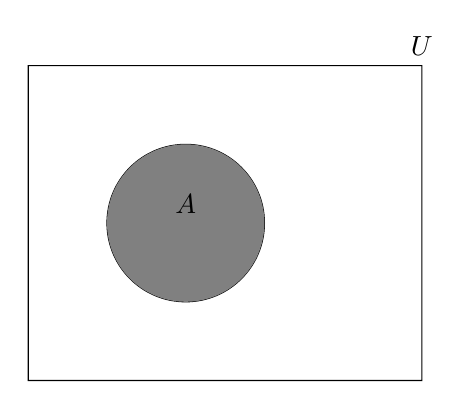
\begin{tikzpicture}[fill=gray]
		 		\draw (0,0) circle (1) (0,0)  node [text=black,above] {$A$}
		 		(-2,-2) rectangle (3,2) node [text=black,above] {$U$};
		 		\fill (0,0) circle (1) (0,0) node [text=black,above] {$A$};
		 		
		 	\end{tikzpicture} 
		 	\item This Venn diagram highlights $(A\cap B)^c$, i.e. the shaded area is the complement of the intersection of $A$ and $B$.\\
		 	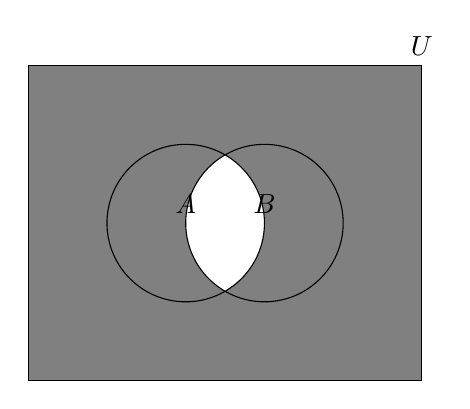
\begin{tikzpicture}
		 		\filldraw[fill=gray] (-2,-2) rectangle (3,2) node [text=black,above] {$U$};
		 		\scope % A \cap B
		 		\clip (0,0) circle (1);
		 		\fill[white] (1,0) circle (1);
		 		\endscope
		 		% outline
		 		\draw (0,0) circle (1) node [text=black,above] {$A$}
		 		(1,0) circle (1) node [text=black,above] {$B$};
		 	\end{tikzpicture}
		 \end{enumerate}
		 
		 
		 
		\subsection{Some useful identities}
		 There are certain identities that are useful when working with sets. For us, these identities establish connections between the three set operations that we have mentioned in this note: union, intersection and taking (relative) complements. \\

		 
		 Here is a list of useful identities: \begin{enumerate}
		 	\item  $(A^c)^c=A$
		 	\item $(A\cap B)^c = A^c \cup B^c$
		 	\item $(A\cup B)^c = A^c \cap B^c$
		 	\item $(\bigcap_{i=1}^n A_i)^c = \bigcup_{i=1}^n A_i^c$
		 	\item $(\bigcup_{i=1}^n A_i )^c= \bigcap_{i=1}^n A_i^c$
		 	\item $(\bigcap_{i=1}^\infty A_i)^c = \bigcup_{i=1}^\infty A_i^c$
		 	\item $(\bigcup_{i=1}^\infty A_i)^c = \bigcap_{i=1}^\infty A_i^c$
		 \end{enumerate} 
		
		Venn diagrams can be useful in establishing some of these identities: Draw a Venn diagram for the set on the left hand side of the equation, do the same for the set on the right hand side of the equation and if the shaded regions are the same then the equation holds! 
		 
		
		 \section{The role of sets in Stat 400}
		 
		 As we discussed above, the idea for us that sets provide a \textit{useful language for discussing events and combinations of events}. The idea is that  for a given experiment that we are interested in, the set of all possible outcomes will act as the universal set, i.e. the role of the universal set will always be played by the sample space. Events can now be described as \textit{subsets} of the sample space. \\
		 
		 
		 Consider rolling a die. The possible outcomes are now $1, 2,3,4,5,6$. The set that contains these outcomes is now $\Omega=\{ 1,2,3,4,5,6 \}$ . Examples of events include \begin{enumerate}
		 		\item $\{1,2\}$: you see either a 1 or a 2 when the die is rolled.
		 		\item $\{4,5,6\}$: you see either a 4, a 5, or a 6 when the die is rolled.
		 		\item $\emptyset$: the empty or null event indicates the (im)possibility that nothing happens when you conduct the experiment.
		 		\item $\{1,2,3,4,5,6\}$ you see either a 1 or a 2 or 3 or a 4 or a 5 or a 6 when the die is rolled
		 		\end{enumerate}
		 
		 \textbf{In general given an event $A$ lists a collection of possible outcomes of the experiment of interest  and $P(A)$ denotes the probability that an outcome listed in $A$ takes place.} 

    \section{Cardinality}

    The last concept we will need from set theory is that of cardinality. Cardinality aims to measure how many elements are in a set. In order to define what it means for two sets to have the same cardinality, we need the notion of a bijection first.

    Recall that a function $f: A \rightarrow B$ is a \textit{bijection} if:
    \begin{enumerate}
        \item it is \textit{surjective} (or \textit{onto}), i.e for any $b\in B$ there is some $a \in A$ such that $f(a) = b$.
        \item it is \textit{injective} (or \textit{one-to-one}), i.e for any $a_1, a_2$ in $A$ with $f(a_1) = f(a_2)$, we have $a_1 = a_2$.
    \end{enumerate}
    
    \begin{defn}
        Two sets $A$ and $B$ have the same cardinality (denoted by $|A| = |B|$) if and only if there is a \textit{bijection} between $A$ and $B$.
    \end{defn}

   

    So $|A| = |B|$ implies that each element in $A$ can be paired with a unique element of $B$. \textit{Thus the number of elements must be the same as that of $B$.}
    \begin{ex}
        \begin{enumerate}
            \item Let $2 \mathbb{N} = \left\{2,4,6,8,10,\ldots\right\}$. Then
            \[
            |2\mathbb{N}| = |\mathbb{N}|
            \]
            The function $f: \mathbb{N} \rightarrow \mathbb{N}$
            \[
            f(x) = 2x
            \]
            is a bijection.
            \item The interval $(-\frac{\pi}{2}, \frac{\pi}{2})$ has the same cardinality as $\mathbb{R}$. The function $f: (-\frac{\pi}{2}, \frac{\pi}{2}) \rightarrow \mathbb{R}$ where
            \[
            f(x) = \tan(x)
            \]
            is a bijection.
        \end{enumerate}
    \end{ex}

    Note that in the example above, $2\mathbb{N} \subseteq \mathbb{N}$ and $\mathbb{N} \neq 2 \mathbb{N}$ (sometimes denoted as $2\mathbb{N} \varsubsetneq \mathbb{N}$), and $(-\frac{\pi}{2}, \frac{\pi}{2}) \varsubsetneq \mathbb{R}$. It turns out that this happens when we have infinite sets. This is not the case with finite sets.

    In our context, the notions of \textit{countable} and \textit{uncountable} sets are important: problems involving countable sets are usually handled using sums (and matrices), while those involving uncountable sets use integrals.

    \begin{defn}
        A set $A$ is said to be \textit{countable} if it is empty or there is a \textit{surjection}, or surjective function $f: \mathbb{N} \rightarrow A$. A set is \textit{uncountable} if it is not countable.
    \end{defn}
    Note that \textit{finite sets} are countable too. For example, if 
    \[
    A = \{0,1,2,3,4,5\}
    \]
    \[
    f: \mathbb{N} \rightarrow A
    \hspace{1cm}
    f(x) = x\mod6
    \]
    (where $x\mod6$ is the remainder when you divide $x$ by 6).
    
    We differentiate between countable sets that are finite and countable sets that are infinite by calling sets that are countable and infinite \textit{countably infinite}.

    Recognizing a set as finite or infinite is usually fairly straightforward. However recognizing an infinite set as countably infinite or uncountable can be difficult. Here, I will list out the most common countably infinite and uncountable sets.

    \textbf{Countable sets}
    \begin{itemize}
        \item $\mathbb{N}$
        \item $\mathbb{Q}$
        \item If $A_1, A_2, \ldots, A_n$ are countable, then $A=A_1 \times \ldots \times A_n$ (also written $\prod_{i=1}^n A_i$, the set of all ordered $n$-tuples) is also countable.
    \end{itemize}

    \textbf{Uncountable sets}
    \begin{itemize}
        \item $\mathbb{R}$
        \item Any nontrivial interval, e.g $(a,b)$ where $a < b$
        \item The irrationals
        \item If $A_1, \ldots, A_n$ are uncountable, then so is $A = A_1 \times \ldots \times A_n$.
    \end{itemize}

    If you are up for a challenge, see if you can use the following theorem to show that $\mathbb{N}$ and $\mathbb{N} \times \mathbb{N}$ have the same cardinality.

    \begin{thm} \textbf{Schr\"{o}der-Bernstein theorem.}
    
        Suppose that there are one-to-one functions $f: A \rightarrow B$ and $g: B\rightarrow A$. Then $|A| = |B|$.
    \end{thm}

\thischapterexercises
    \exerciseitem Use Venn diagrams to determine whether the following relations always hold.
          \begin{enumerate}
              \item $(A \cap B)^c = A^c \cup B^c$
              \item $(A - B) \cap C = (A \cup B) \cap (A \cup C)$
              \item $(A - B) \cap (B- A) = \emptyset$
          \end{enumerate}
    \\
    \exerciseitem Let $A = \{3n : n \in \N\}$. Find a bijection from $A$ to $\N$.\\
    
    \exerciseitem Let $\Omega = \N$, $A = 2\N$, $B = 3\N$. Describe the following sets.
    \begin{enumerate}
        \item $A \cap B$
        \item $A \cup B$
        \item $A - B$
        \item $B - A$
    \end{enumerate} \\
    
    \exerciseitem Let $\Omega = \{1,2,3,4,5,6\}$, $A = \{2,3,5\}$, $B = \{2,4,6\}$. Compute:
    \begin{enumerate}
        \item $A \cup B$
        \item $A \cap B$
        \item $A - B$
        \item $B - A$
    \end{enumerate}
\end{appendices}